\documentclass{article}

\usepackage{amsthm}
\usepackage{amsmath}
\usepackage{cite}
\usepackage{listings}
\usepackage{multicol}
\usepackage{url}
\usepackage{graphicx}
\graphicspath{ {./imgs/} }

\setlength{\parindent}{4em}
\setlength{\parskip}{1em}


\begin{document}

\pagenumbering{gobble}

\begin{center}
  \textbf{Project Final Report}

  \textit{Derick Anderson and Harshitha Bhaskar, Blackboard: AndersonBhaskar}
\end{center}

\section*{Idea}

The core idea of the project is to develop a journaling tool for managing your
reading. Functionality will include, for example, the ability to track your
progress through books from want-to-read to finished, write reviews of books,
and organize books by author and series. To support said functionality will
require a data model for books, authors, reading lists, etc.

We love to read, but lose track of all the information to do with our
reading. It is great to be able to look forward to the things you want to read,
look back on the things you’ve read, and organize your thoughts about your
reading.

\section*{UML and EER Diagrams}

Due to the way that \LaTeX \ distributes figures
the diagrams are not located exactly at this point,
but they are contained in the document.
They are unchanged from the progress report
because while the schema has been updated somewhat
(with new triggers, constraints)
the structure of our tables has not changed.

\begin{figure}[h]
  \centering
  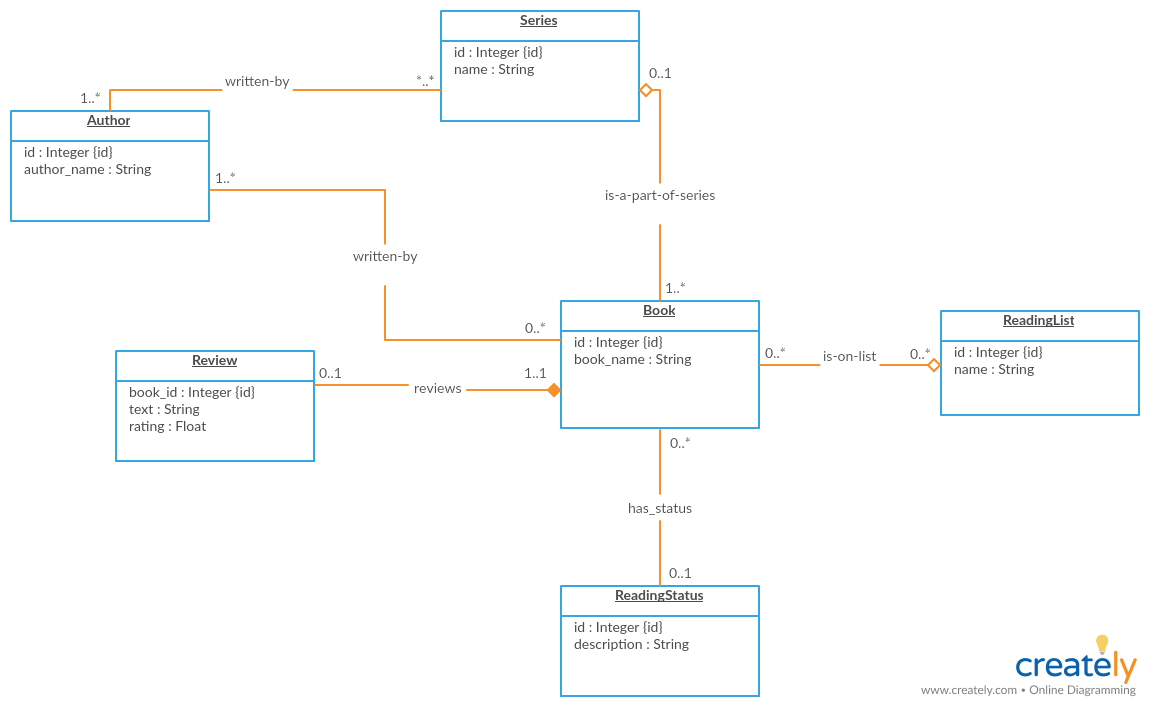
\includegraphics[width=\textwidth]{uml}
  \caption{UML Diagram}
\end{figure}

\begin{figure}[h]
  \centering
  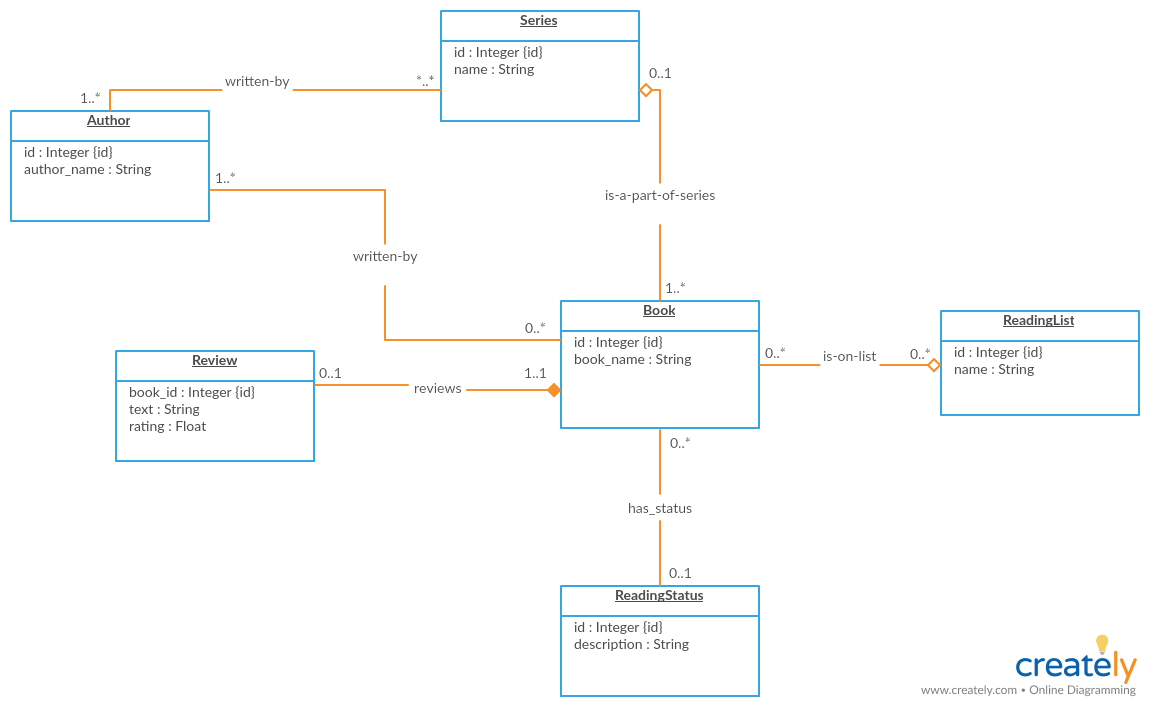
\includegraphics[width=\textwidth]{uml}
  \caption{EER Diagram}
\end{figure}

\section*{User Flow}

% TODO: Harshitha

\section*{Technical Specifications}

We used Python 3.7 as our frontend and backend language,
its SQLAlchemy library with the
PyMySQL \footnote{https://github.com/PyMySQL/mysqlclient-python}
connector,
the Tkinter GUI framework,
and the pytest testing framework.
We used the MySQL database with the InnoDB engine.
Note that we will utilize only the core features of SQLAlchemy:
most notably we will not utilize its ORM functionality.

We will target Ubuntu 18.10, MacOS 10.14, and MySQL 14.14.

\section*{Lessons Learned}

\section*{Future Work}

\end{document}
%%% Local Variables:
%%% mode: latex
%%% TeX-master: t
%%% End:
